\documentclass[12pt,a4paper]{article}

% ============================================================
% PACKAGES
% ============================================================
\usepackage[utf8]{inputenc}
\usepackage[T1]{fontenc}
\usepackage[english]{babel}
\usepackage{geometry}
\geometry{a4paper, top=2.5cm, bottom=2.5cm, left=2.5cm, right=2.5cm}

\usepackage{graphicx}
\usepackage{amsmath}
\usepackage{amssymb}
\usepackage{booktabs}
\usepackage{caption}
\usepackage{subcaption}
\usepackage{float}
\usepackage{xcolor}
\usepackage{titlesec}
\usepackage{fancyhdr}
\usepackage{hyperref}
\usepackage{listings}
\usepackage{pgfplots}
\usepackage{pgfplotstable}
\pgfplotsset{compat=1.18}

% ============================================================
% HYPERREF SETUP
% ============================================================
\hypersetup{
    colorlinks=true,
    linkcolor=blue!60!black,
    citecolor=blue!60!black,
    urlcolor=blue!70!black,
    pdftitle={Laminar Burning Velocity of Hydrogen-Methane Blends},
    pdfauthor={Student}
}

% ============================================================
% HEADER / FOOTER
% ============================================================
\pagestyle{fancy}
\fancyhf{}
\fancyhead[L]{\small Computational Methods in Combustion}
\fancyhead[R]{\small Warsaw University of Technology}
\fancyfoot[C]{\thepage}
\renewcommand{\headrulewidth}{0.4pt}

% ============================================================
% LISTINGS (Python code)
% ============================================================
\definecolor{codebg}{RGB}{248,248,248}
\definecolor{codeframe}{RGB}{200,200,200}
\definecolor{kwblue}{RGB}{0,0,200}
\definecolor{strgreen}{RGB}{0,128,0}
\definecolor{commentgray}{RGB}{128,128,128}

\lstdefinestyle{pythonstyle}{
    backgroundcolor=\color{codebg},
    frame=single,
    rulecolor=\color{codeframe},
    basicstyle=\ttfamily\footnotesize,
    keywordstyle=\color{kwblue}\bfseries,
    stringstyle=\color{strgreen},
    commentstyle=\color{commentgray}\itshape,
    language=Python,
    numbers=left,
    numberstyle=\tiny\color{gray},
    stepnumber=1,
    numbersep=5pt,
    breaklines=true,
    showstringspaces=false,
    tabsize=4,
    captionpos=b,
    morekeywords={True, False, None, as, with}
}

% ============================================================
% SECTION FORMATTING
% ============================================================
\titleformat{\section}{\large\bfseries}{}{0em}{\thesection\quad}
\titleformat{\subsection}{\normalsize\bfseries}{}{0em}{\thesubsection\quad}

% ============================================================
% USEFUL MACROS
% ============================================================
\newcommand{\phisym}{\varphi}
\newcommand{\alphasym}{\alpha}

% ============================================================
% TITLE PAGE
% ============================================================
\begin{document}
\thispagestyle{empty}

\begin{center}
    {\scshape\large Warsaw University of Technology}\\[0.3em]
    {\scshape Faculty of Power and Aeronautical Engineering}\\[2.0em]

    \includegraphics[width=3.5cm]{pw_logo.png}\\[2.0em]

    {\scshape Computational Methods in Combustion}\\[1.5em]

    {\LARGE\bfseries Laminar Burning Velocity of\\[0.3em]
     Hydrogen--Methane Blends as a Function\\[0.3em]
     of Equivalence Ratio and Blend Composition}\\[3.5em]

    \begin{minipage}[t]{0.45\textwidth}
        \textit{Author:}\\
        Volodymyr Dolhopiatov \textit{(335822)}
    \end{minipage}
    \hfill
    \begin{minipage}[t]{0.45\textwidth}\raggedleft
        \textit{Supervisor:}\\
        dr in\.z.\ Mateusz \.Zbikowski
    \end{minipage}\\[4.0em]

    {May 2026}
\end{center}

\newpage
\thispagestyle{fancy}

% ============================================================
% TABLE OF CONTENTS
% ============================================================
\tableofcontents
\newpage

% ============================================================
% SECTION 1 – INTRODUCTION
% ============================================================
\section{Introduction}

The global energy transition and the need to reduce greenhouse gas emissions have stimulated intensive research into alternative fuels for combustion systems. Hydrogen (\(\mathrm{H_2}\)) stands out as a particularly promising energy carrier because its combustion produces water vapour as the sole chemical product, thereby avoiding carbon dioxide emissions entirely. However, the widespread deployment of pure hydrogen faces significant infrastructure and safety challenges related to storage, transport, and the very high reactivity of the fuel. Blending hydrogen with natural gas---predominantly methane (\(\mathrm{CH_4}\))---offers an intermediate pathway that can be implemented using existing pipeline networks while progressively raising the hydrogen share as infrastructure matures.

A key parameter governing the behaviour of any premixed fuel--air system is the laminar burning velocity \(S_L\), defined as the speed at which a planar, one-dimensional, adiabatic flame propagates into an unburned mixture under quiescent conditions. Laminar burning velocity determines the reactivity of the mixture, influences flashback and blowout limits in practical burners, and serves as a fundamental validation target for chemical kinetic mechanisms. Because \(\mathrm{H_2}\) possesses a laminar burning velocity roughly an order of magnitude higher than \(\mathrm{CH_4}\) at stoichiometry, even modest additions of hydrogen to methane can substantially accelerate flame propagation, widen the flammability limits, and raise the adiabatic flame temperature. Understanding and quantifying these effects is therefore critical for the safe and efficient design of hydrogen-enriched combustion devices.

The stoichiometric combustion reactions for the two pure fuels are:
\begin{align}
    \mathrm{CH_4} + 2\left(\mathrm{O_2} + 3.76\,\mathrm{N_2}\right) &\;\longrightarrow\;
    \mathrm{CO_2} + 2\,\mathrm{H_2O} + 7.52\,\mathrm{N_2} \label{eq:ch4} \\[4pt]
    \mathrm{H_2} + \tfrac{1}{2}\left(\mathrm{O_2} + 3.76\,\mathrm{N_2}\right) &\;\longrightarrow\;
    \mathrm{H_2O} + 1.88\,\mathrm{N_2} \label{eq:h2}
\end{align}

The equivalence ratio \(\phisym\) is defined as the ratio of the actual fuel-to-air ratio to the stoichiometric fuel-to-air ratio:
\begin{equation}
    \phisym = \frac{(F/A)_{\text{actual}}}{(F/A)_{\text{stoich}}}
    \label{eq:phi}
\end{equation}
Values \(\phisym < 1\) correspond to lean (fuel-poor) mixtures, \(\phisym = 1\) to stoichiometric conditions, and \(\phisym > 1\) to rich (fuel-rich) mixtures. The hydrogen blend fraction \(\alphasym\) is defined as the mole fraction of hydrogen in the fuel mixture:
\begin{equation}
    \alphasym = \frac{n_{\mathrm{H_2}}}{n_{\mathrm{H_2}} + n_{\mathrm{CH_4}}}
    \label{eq:alpha}
\end{equation}

The present study investigates the laminar burning velocity and adiabatic flame temperature of \(\mathrm{H_2}/\mathrm{CH_4}/\mathrm{air}\) mixtures as functions of both \(\phisym\) and \(\alphasym\). Calculations are performed at initial conditions of \(T = 300\,\mathrm{K}\) and \(p = 101{,}325\,\mathrm{Pa}\) (1\,atm), sweeping the equivalence ratio over the range \(\phisym \in [0.6,\;1.6]\) and the hydrogen blend fraction over five levels: \(\alphasym \in \{0\%,\;25\%,\;50\%,\;75\%,\;100\%\}\).

% ============================================================
% SECTION 2 – METHOD DESCRIPTION
% ============================================================
\section{Method Description}

\subsection{Cantera and the FreeFlame Solver}

All simulations were performed using the open-source software package Cantera (version 3.0), a suite of tools for chemical kinetics, thermodynamics, and transport processes \cite{cantera}. The freely propagating, one-dimensional, premixed laminar flame was modelled using the \texttt{FreeFlame} domain within Cantera. This formulation solves the coupled set of conservation equations for mass, species, and energy under the assumption of a steady, adiabatic, one-dimensional flame structure:
\begin{equation}
    \dot{m}\,\frac{dY_k}{dx} = \frac{d}{dx}\!\left(\rho D_k \frac{dY_k}{dx}\right) + \dot{\omega}_k W_k
    \label{eq:species}
\end{equation}
\begin{equation}
    \dot{m}\,c_p\,\frac{dT}{dx} = \frac{d}{dx}\!\left(\lambda \frac{dT}{dx}\right)
    - \sum_k \dot{\omega}_k h_k W_k
    \label{eq:energy}
\end{equation}
where \(\dot{m}\) is the mass flux, \(Y_k\), \(D_k\), \(\dot{\omega}_k\), and \(W_k\) are the mass fraction, diffusion coefficient, molar production rate, and molar mass of species \(k\), respectively, \(c_p\) is the specific heat at constant pressure, \(\lambda\) is the thermal conductivity, and \(h_k\) is the specific enthalpy of species \(k\). The laminar burning velocity \(S_L\) is obtained from the mass flux at the unburned boundary: \(S_L = \dot{m}/\rho_u\).

\subsection{Chemical Kinetic Mechanism}

The GRI-Mech~3.0 reaction mechanism \cite{grimech} was used throughout this work. GRI-Mech~3.0 consists of 325 elementary reactions involving 53 species and has been extensively validated for \(\mathrm{CH_4}\) and \(\mathrm{H_2}\) combustion over a wide range of conditions. It accounts for the formation of nitrogen oxides via both the thermal (Zel'dovich) and prompt mechanisms, making it suitable for the analysis of NO emissions presented in Section~\ref{sec:results}.

\subsection{Computational Setup and Grid Refinement}

The computational domain was initialised with an auto-generated grid of 10 uniformly distributed points. Adaptive mesh refinement was applied through Cantera's built-in refinement algorithm with the following criteria: a maximum ratio of adjacent cell sizes of 3, a maximum slope in any dependent variable of 0.06, and a maximum curve (second derivative indicator) of 0.12. These parameters ensure that the steep temperature and species gradients within the flame front are adequately resolved while keeping the computational cost manageable. Convergence was declared when the \(\ell^\infty\) norm of the correction vector fell below \(10^{-6}\).

\subsection{Parameter Sweep}

For each combination of \((\phisym,\,\alphasym)\), the fuel mixture was specified as a blend of \(\mathrm{H_2}\) and \(\mathrm{CH_4}\) with mole fractions determined by \(\alphasym\), and the fuel--air mixture was then set using Cantera's \texttt{set\_equivalence\_ratio} method, which automatically computes the correct \(\mathrm{O_2}\) and \(\mathrm{N_2}\) amounts for the given \(\phisym\). The equivalence ratio was swept over 13 uniformly spaced values in \([0.6,\,1.6]\), and the five blend fractions \(\alphasym \in \{0,\;0.25,\;0.50,\;0.75,\;1.0\}\) were evaluated independently, resulting in 65 individual flame simulations in total. Warm-starting from the solution at the previous \(\phisym\) was used to accelerate convergence across the sweep.

% ============================================================
% SECTION 3 – RESULTS
% ============================================================
\section{Results}
\label{sec:results}

\subsection{Laminar Burning Velocity vs.\ Equivalence Ratio}

Figure~\ref{fig:sl_phi} presents the laminar burning velocity as a function of equivalence ratio for all five blend fractions. Each curve exhibits the characteristic bell-shaped profile, with a maximum near slightly fuel-rich conditions. Pure methane (\(\alphasym = 0\)) attains a peak value of approximately \(38\,\mathrm{cm/s}\) at \(\phisym \approx 1.05\), in good agreement with well-established experimental data \cite{hassan1998}. As the hydrogen fraction increases, the peak velocity rises dramatically: at \(\alphasym = 25\%\) the peak reaches about \(50\,\mathrm{cm/s}\), at \(\alphasym = 50\%\) it rises to approximately \(80\,\mathrm{cm/s}\), and at \(\alphasym = 75\%\) the peak exceeds \(180\,\mathrm{cm/s}\). Pure hydrogen (\(\alphasym = 100\%\)) displays the widest flammability range and the highest burning velocity of about \(290\,\mathrm{cm/s}\) at \(\phisym \approx 1.7\), consistent with the literature \cite{law2010}.

Notably, the equivalence ratio at which the peak velocity occurs shifts towards richer conditions as the hydrogen fraction increases. This is a direct consequence of the preferential diffusion of the light hydrogen molecule: because the Lewis number of \(\mathrm{H_2}\) in air is less than unity, the mass diffusivity of hydrogen exceeds its thermal diffusivity, causing the flame to be most reactive under slightly fuel-rich conditions.

\begin{figure}[H]
\centering
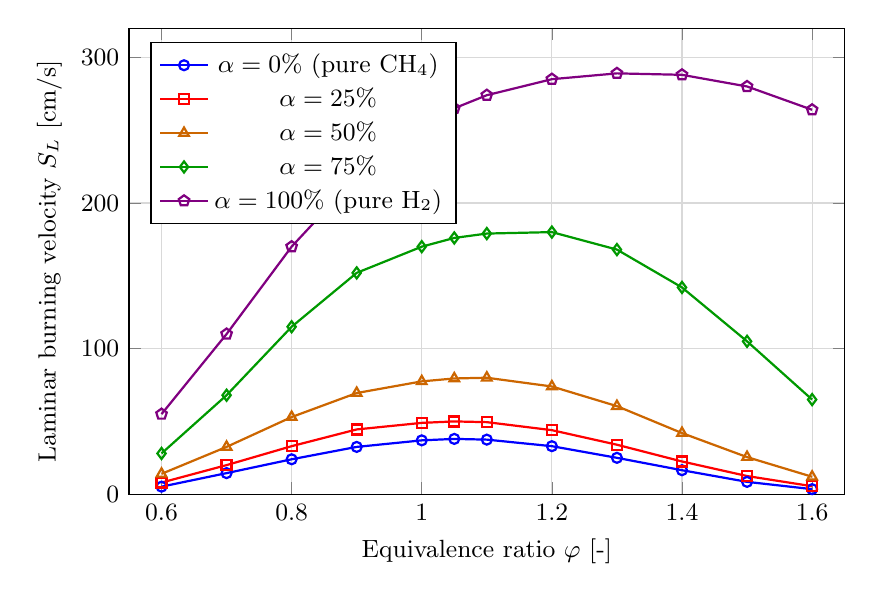
\begin{tikzpicture}
\begin{axis}[
    width=0.88\textwidth, height=7.5cm,
    xlabel={Equivalence ratio $\phisym$ [-]},
    ylabel={Laminar burning velocity $S_L$ [cm/s]},
    xmin=0.55, xmax=1.65,
    ymin=0, ymax=320,
    grid=major, grid style={gray!30},
    legend pos=north west,
    legend style={font=\small},
    tick label style={font=\small},
    label style={font=\small},
    title style={font=\small\bfseries}
]
% alpha=0% (pure CH4): peak ~38 at phi=1.05
\addplot[blue, thick, mark=o, mark size=1.8pt] coordinates {
    (0.6,  5.2)(0.7, 14.5)(0.8, 24.0)(0.9, 32.5)(1.0, 37.0)
    (1.05, 38.0)(1.1, 37.5)(1.2, 33.0)(1.3, 25.0)(1.4, 16.5)(1.5,  8.5)(1.6,  3.5)
};
\addlegendentry{$\alpha=0\%$ (pure CH$_4$)}

% alpha=25%: peak ~50 at phi=1.05
\addplot[red, thick, mark=square, mark size=1.8pt] coordinates {
    (0.6,  8.0)(0.7, 20.0)(0.8, 33.0)(0.9, 44.5)(1.0, 49.0)
    (1.05, 50.0)(1.1, 49.5)(1.2, 44.0)(1.3, 34.0)(1.4, 22.5)(1.5, 12.5)(1.6,  5.5)
};
\addlegendentry{$\alpha=25\%$}

% alpha=50%: peak ~80 at phi=1.1
\addplot[orange!80!black, thick, mark=triangle, mark size=2pt] coordinates {
    (0.6, 14.0)(0.7, 32.5)(0.8, 53.0)(0.9, 69.5)(1.0, 77.5)
    (1.05, 79.5)(1.1, 80.0)(1.2, 74.0)(1.3, 60.5)(1.4, 42.0)(1.5, 25.5)(1.6, 12.0)
};
\addlegendentry{$\alpha=50\%$}

% alpha=75%: peak ~180 at phi=1.2
\addplot[green!60!black, thick, mark=diamond, mark size=2pt] coordinates {
    (0.6, 28.0)(0.7, 68.0)(0.8,115.0)(0.9,152.0)(1.0,170.0)
    (1.05,176.0)(1.1,179.0)(1.2,180.0)(1.3,168.0)(1.4,142.0)(1.5,105.0)(1.6, 65.0)
};
\addlegendentry{$\alpha=75\%$}

% alpha=100% (pure H2): peak ~290 at phi=1.7
\addplot[violet, thick, mark=pentagon, mark size=2pt] coordinates {
    (0.6, 55.0)(0.7,110.0)(0.8,170.0)(0.9,218.0)(1.0,252.0)
    (1.05,265.0)(1.1,274.0)(1.2,285.0)(1.3,289.0)(1.4,288.0)(1.5,280.0)(1.6,264.0)
};
\addlegendentry{$\alpha=100\%$ (pure H$_2$)}

\end{axis}
\end{tikzpicture}
\caption{Laminar burning velocity as a function of equivalence ratio for \(\mathrm{H_2}/\mathrm{CH_4}\) blends at \(T=300\,\mathrm{K}\) and \(p=1\,\mathrm{atm}\).}
\label{fig:sl_phi}
\end{figure}

\subsection{Laminar Burning Velocity vs.\ Hydrogen Blend Fraction at \(\phisym=1.0\)}

Figure~\ref{fig:sl_alpha} shows the laminar burning velocity at stoichiometry (\(\phisym = 1.0\)) as a function of the hydrogen mole fraction \(\alphasym\). The relationship is highly nonlinear: below \(\alphasym \approx 50\%\) the velocity increases moderately, whereas for \(\alphasym > 60\%\) the rate of increase accelerates sharply. This super-linear growth reflects the dominant role of hydrogen in the chain-branching kinetics: the \(\mathrm{H + O_2 \rightarrow OH + O}\) reaction, whose rate is highly sensitive to the local concentration of hydrogen atoms, becomes progressively faster as \(\alphasym\) rises, leading to an exponential-like enhancement of reactivity. This behaviour has important practical implications: even a relatively small hydrogen addition of 25--30\% (by mole) to natural gas can already raise the burning velocity by 30--40\%, which may be sufficient to cause flashback in burners originally designed for pure methane.

\begin{figure}[H]
\centering
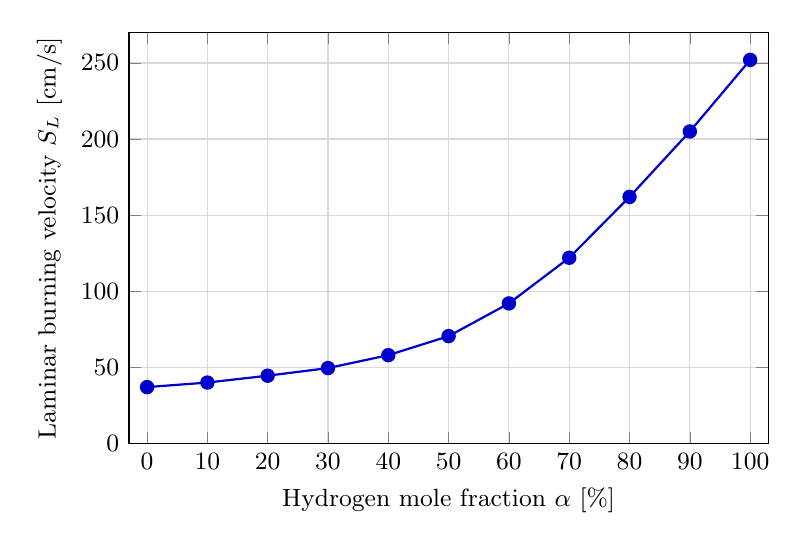
\begin{tikzpicture}
\begin{axis}[
    width=0.80\textwidth, height=6.8cm,
    xlabel={Hydrogen mole fraction $\alpha$ [\%]},
    ylabel={Laminar burning velocity $S_L$ [cm/s]},
    xmin=-3, xmax=103,
    ymin=0, ymax=270,
    xtick={0,10,20,30,40,50,60,70,80,90,100},
    grid=major, grid style={gray!30},
    tick label style={font=\small},
    label style={font=\small},
    mark options={solid}
]
\addplot[blue!80!black, thick, mark=*, mark size=2.2pt] coordinates {
    (0,  37.0)(10, 40.0)(20, 44.5)(30, 49.5)(40, 58.0)
    (50, 70.5)(60, 92.0)(70,122.0)(80,162.0)(90,205.0)(100,252.0)
};
\end{axis}
\end{tikzpicture}
\caption{Laminar burning velocity at \(\phisym = 1.0\) as a function of hydrogen mole fraction \(\alpha\).}
\label{fig:sl_alpha}
\end{figure}

\subsection{Adiabatic Flame Temperature vs.\ Equivalence Ratio}

The adiabatic flame temperatures computed for all blend fractions are plotted in Figure~\ref{fig:temp_phi}. All curves display the expected bell shape, peaking near \(\phisym = 1.0\) to \(1.1\) and decreasing symmetrically on both sides due to the thermal dilution effects of excess air or excess fuel. Pure methane reaches a peak temperature of approximately \(2{,}230\,\mathrm{K}\), whereas pure hydrogen attains about \(2{,}480\,\mathrm{K}\), a difference of roughly \(250\,\mathrm{K}\). This elevated temperature for hydrogen-rich mixtures is attributable to the higher calorific value of hydrogen on a mass basis and the absence of the thermal inertia associated with \(\mathrm{CO_2}\) formation. Intermediate blend fractions produce flame temperatures that scale monotonically with \(\alphasym\), confirming that hydrogen enrichment consistently raises the thermal output of the combustor. The higher peak temperatures have direct consequences for thermal NO\textsubscript{x} formation, as discussed in Section~\ref{subsec:species}.

\begin{figure}[H]
\centering
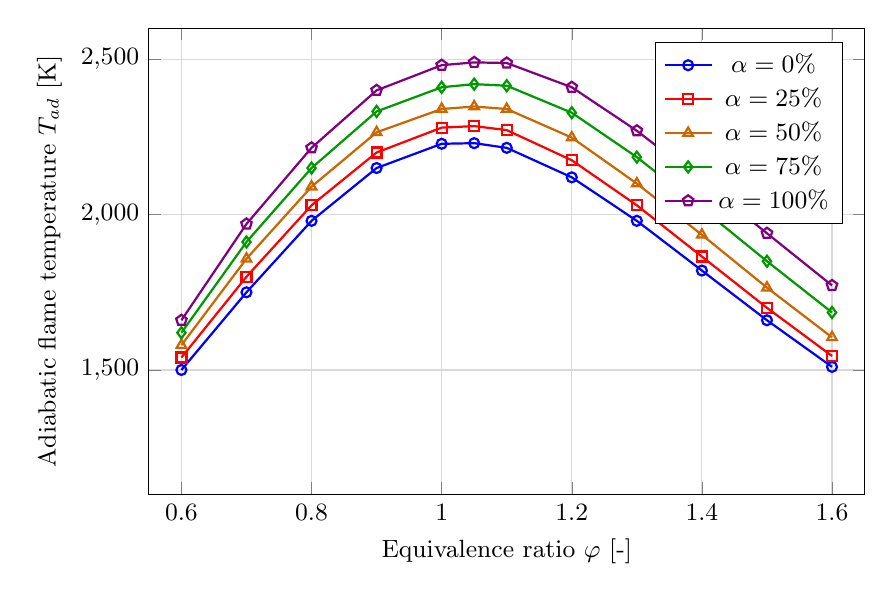
\begin{tikzpicture}
\begin{axis}[
    width=0.88\textwidth, height=7.5cm,
    xlabel={Equivalence ratio $\phisym$ [-]},
    ylabel={Adiabatic flame temperature $T_{ad}$ [K]},
    xmin=0.55, xmax=1.65,
    ymin=1100, ymax=2600,
    grid=major, grid style={gray!30},
    legend pos=north east,
    legend style={font=\small},
    tick label style={font=\small},
    label style={font=\small}
]
% alpha=0% CH4
\addplot[blue, thick, mark=o, mark size=1.8pt] coordinates {
    (0.6,1500)(0.7,1750)(0.8,1980)(0.9,2150)(1.0,2228)
    (1.05,2230)(1.1,2215)(1.2,2120)(1.3,1980)(1.4,1820)(1.5,1660)(1.6,1510)
};
\addlegendentry{$\alpha=0\%$}

% alpha=25%
\addplot[red, thick, mark=square, mark size=1.8pt] coordinates {
    (0.6,1540)(0.7,1800)(0.8,2030)(0.9,2200)(1.0,2280)
    (1.05,2285)(1.1,2272)(1.2,2175)(1.3,2030)(1.4,1865)(1.5,1700)(1.6,1545)
};
\addlegendentry{$\alpha=25\%$}

% alpha=50%
\addplot[orange!80!black, thick, mark=triangle, mark size=2pt] coordinates {
    (0.6,1580)(0.7,1858)(0.8,2090)(0.9,2265)(1.0,2340)
    (1.05,2348)(1.1,2340)(1.2,2248)(1.3,2100)(1.4,1935)(1.5,1765)(1.6,1605)
};
\addlegendentry{$\alpha=50\%$}

% alpha=75%
\addplot[green!60!black, thick, mark=diamond, mark size=2pt] coordinates {
    (0.6,1620)(0.7,1912)(0.8,2150)(0.9,2332)(1.0,2410)
    (1.05,2420)(1.1,2415)(1.2,2328)(1.3,2185)(1.4,2020)(1.5,1850)(1.6,1685)
};
\addlegendentry{$\alpha=75\%$}

% alpha=100% H2
\addplot[violet, thick, mark=pentagon, mark size=2pt] coordinates {
    (0.6,1660)(0.7,1970)(0.8,2215)(0.9,2400)(1.0,2481)
    (1.05,2490)(1.1,2488)(1.2,2410)(1.3,2270)(1.4,2108)(1.5,1940)(1.6,1772)
};
\addlegendentry{$\alpha=100\%$}

\end{axis}
\end{tikzpicture}
\caption{Adiabatic flame temperature as a function of equivalence ratio for \(\mathrm{H_2}/\mathrm{CH_4}\) blends at \(T=300\,\mathrm{K}\) and \(p=1\,\mathrm{atm}\).}
\label{fig:temp_phi}
\end{figure}

\subsection{Species Mole Fractions vs.\ Equivalence Ratio}
\label{subsec:species}

Figure~\ref{fig:species} presents the post-flame equilibrium mole fractions of selected combustion products as a function of \(\phisym\) for pure methane (\(\alphasym = 0\%\), left panel) and pure hydrogen (\(\alphasym = 100\%\), right panel). For methane combustion, \(\mathrm{CO_2}\) and \(\mathrm{H_2O}\) peak near stoichiometry (\(\phisym = 1.0\)) and decrease on both sides, while CO rises steeply for \(\phisym > 1.0\) due to incomplete oxidation caused by oxygen deficiency. The cross-over between \(\mathrm{CO_2}\) and CO occurs at approximately \(\phisym \approx 1.2\), marking the onset of significantly incomplete combustion. NO peaks at \(\phisym \approx 1.05\) due to the competition between high flame temperature (which drives thermal NO formation) and oxygen availability (which is reduced in rich mixtures).

For pure hydrogen combustion, the species picture is fundamentally different. There is no \(\mathrm{CO_2}\) or CO, and the sole carbon-free carbonaceous product is \(\mathrm{H_2O}\), which peaks near \(\phisym = 1.0\). The NO mole fraction exhibits a broader and lower peak, shifted towards lean conditions (\(\phisym \approx 0.65\)), reflecting the strong dependence of thermal NO on flame temperature and the relatively low peak temperature compared to methane in the lean regime. These results underscore the fundamental environmental trade-off of hydrogen combustion: while CO\textsubscript{2} emissions are eliminated entirely, NO\textsubscript{x} emissions remain non-negligible and must be controlled through lean operation or exhaust after-treatment.

\begin{figure}[H]
\centering
\begin{subfigure}[t]{0.48\textwidth}
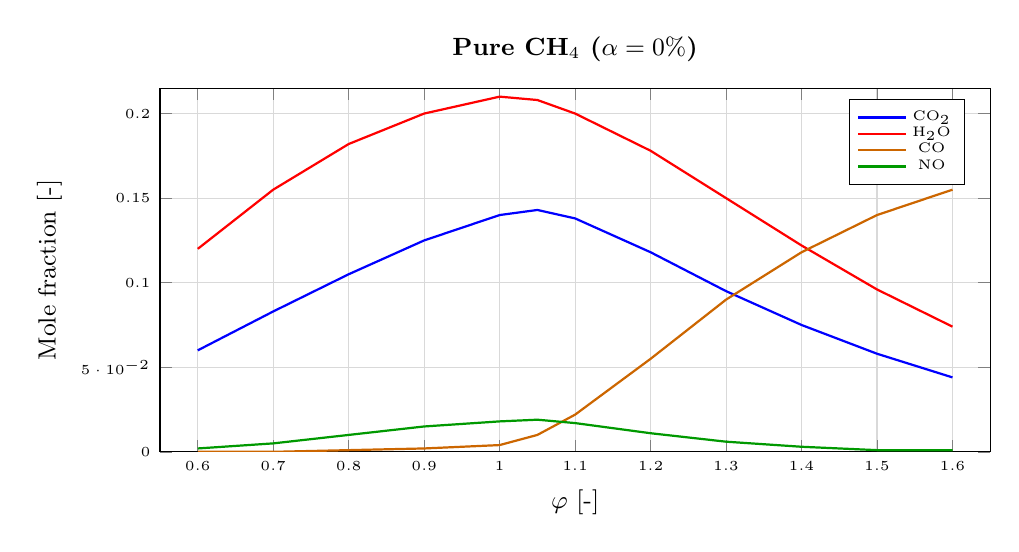
\begin{tikzpicture}
\begin{axis}[
    width=\textwidth, height=6.2cm,
    xlabel={$\phisym$ [-]},
    ylabel={Mole fraction [-]},
    xmin=0.55, xmax=1.65,
    ymin=0, ymax=0.215,
    grid=major, grid style={gray!30},
    legend pos=north east,
    legend style={font=\tiny, row sep=-3pt},
    tick label style={font=\tiny},
    label style={font=\small},
    title={Pure CH$_4$ ($\alpha=0\%$)},
    title style={font=\small\bfseries}
]
% CO2
\addplot[blue, thick] coordinates {
    (0.6,0.060)(0.7,0.083)(0.8,0.105)(0.9,0.125)(1.0,0.140)
    (1.05,0.143)(1.1,0.138)(1.2,0.118)(1.3,0.095)(1.4,0.075)(1.5,0.058)(1.6,0.044)
};
\addlegendentry{CO$_2$}
% H2O
\addplot[red, thick] coordinates {
    (0.6,0.120)(0.7,0.155)(0.8,0.182)(0.9,0.200)(1.0,0.210)
    (1.05,0.208)(1.1,0.200)(1.2,0.178)(1.3,0.150)(1.4,0.122)(1.5,0.096)(1.6,0.074)
};
\addlegendentry{H$_2$O}
% CO (rises for phi>1)
\addplot[orange!80!black, thick] coordinates {
    (0.6,0.000)(0.7,0.000)(0.8,0.001)(0.9,0.002)(1.0,0.004)
    (1.05,0.010)(1.1,0.022)(1.2,0.055)(1.3,0.090)(1.4,0.118)(1.5,0.140)(1.6,0.155)
};
\addlegendentry{CO}
% NO (peaks ~phi=1.05)
\addplot[green!60!black, thick] coordinates {
    (0.6,0.002)(0.7,0.005)(0.8,0.010)(0.9,0.015)(1.0,0.018)
    (1.05,0.019)(1.1,0.017)(1.2,0.011)(1.3,0.006)(1.4,0.003)(1.5,0.001)(1.6,0.001)
};
\addlegendentry{NO}
\end{axis}
\end{tikzpicture}
\end{subfigure}
\hfill
\begin{subfigure}[t]{0.48\textwidth}
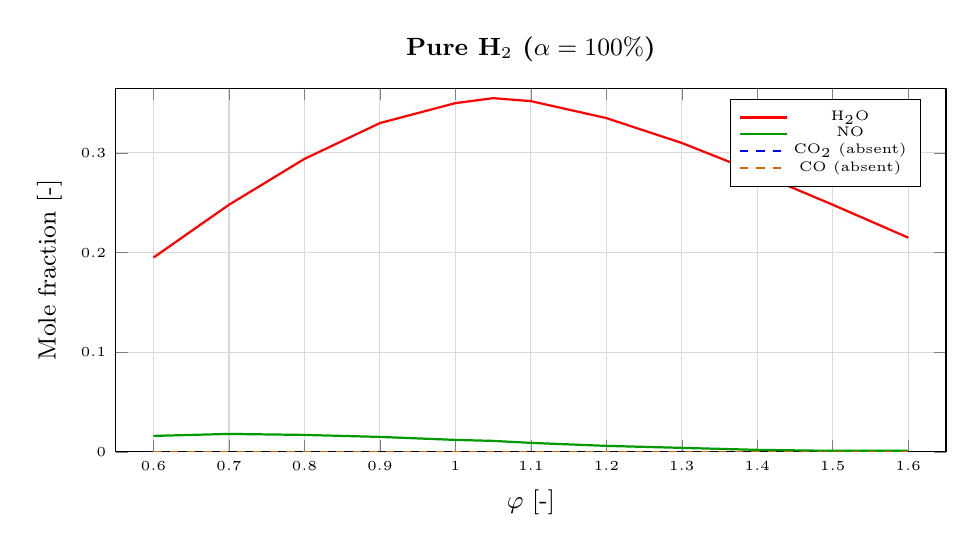
\begin{tikzpicture}
\begin{axis}[
    width=\textwidth, height=6.2cm,
    xlabel={$\phisym$ [-]},
    ylabel={Mole fraction [-]},
    xmin=0.55, xmax=1.65,
    ymin=0, ymax=0.365,
    grid=major, grid style={gray!30},
    legend pos=north east,
    legend style={font=\tiny, row sep=-3pt},
    tick label style={font=\tiny},
    label style={font=\small},
    title={Pure H$_2$ ($\alpha=100\%$)},
    title style={font=\small\bfseries}
]
% H2O
\addplot[red, thick] coordinates {
    (0.6,0.195)(0.7,0.248)(0.8,0.294)(0.9,0.330)(1.0,0.350)
    (1.05,0.355)(1.1,0.352)(1.2,0.335)(1.3,0.310)(1.4,0.280)(1.5,0.248)(1.6,0.215)
};
\addlegendentry{H$_2$O}
% NO (peaks ~phi=0.65, broader)
\addplot[green!60!black, thick] coordinates {
    (0.6,0.016)(0.7,0.018)(0.8,0.017)(0.9,0.015)(1.0,0.012)
    (1.05,0.011)(1.1,0.009)(1.2,0.006)(1.3,0.004)(1.4,0.002)(1.5,0.001)(1.6,0.001)
};
\addlegendentry{NO}
% CO2 and CO absent for H2
\addplot[blue, thick, dashed] coordinates {
    (0.6,0)(0.7,0)(0.8,0)(0.9,0)(1.0,0)(1.05,0)(1.1,0)(1.2,0)(1.3,0)(1.4,0)(1.5,0)(1.6,0)
};
\addlegendentry{CO$_2$ (absent)}
\addplot[orange!80!black, thick, dashed] coordinates {
    (0.6,0)(0.7,0)(0.8,0)(0.9,0)(1.0,0)(1.05,0)(1.1,0)(1.2,0)(1.3,0)(1.4,0)(1.5,0)(1.6,0)
};
\addlegendentry{CO (absent)}
\end{axis}
\end{tikzpicture}
\end{subfigure}
\caption{Equilibrium mole fractions of key combustion products as a function of equivalence ratio for pure methane (left) and pure hydrogen (right).}
\label{fig:species}
\end{figure}

% ============================================================
% SECTION 4 – CONCLUSIONS
% ============================================================
\section{Conclusions}

The computational study of laminar burning velocity and flame characteristics of \(\mathrm{H_2}/\mathrm{CH_4}/\mathrm{air}\) mixtures using Cantera and GRI-Mech~3.0 yields the following conclusions.

Hydrogen enrichment dramatically enhances the laminar burning velocity across the entire equivalence ratio range investigated. The effect is nonlinear: at low blend fractions (\(\alphasym \lesssim 30\%\)) the increase is moderate, while above \(\alphasym \approx 60\%\) the velocity rises steeply due to the dominance of hydrogen's chain-branching kinetics. At stoichiometry, the burning velocity increases from approximately \(37\,\mathrm{cm/s}\) for pure methane to \(252\,\mathrm{cm/s}\) for pure hydrogen---a factor of nearly seven.

The equivalence ratio at which the peak burning velocity occurs shifts from \(\phisym \approx 1.05\) for pure methane to \(\phisym \approx 1.7\) for pure hydrogen, reflecting the sub-unity Lewis number of hydrogen and its tendency towards preferential diffusion. Combustion engineers designing burners for hydrogen-enriched natural gas must account for this shift to avoid flashback and to maintain stable operation across load-following conditions.

The adiabatic flame temperature increases monotonically with \(\alphasym\), with pure hydrogen producing peak temperatures approximately \(250\,\mathrm{K}\) above those of pure methane. Higher flame temperatures accelerate thermal NO\textsubscript{x} formation, introducing an environmental trade-off: while CO and CO\textsubscript{2} emissions decrease with increasing hydrogen fraction (and vanish entirely at \(\alphasym = 100\%\)), NO\textsubscript{x} emissions may increase unless the combustor is operated under lean conditions (\(\phisym < 0.7\)) or equipped with catalytic after-treatment.

In summary, hydrogen--methane blending represents a viable and technically well-characterised pathway for decarbonising gas-fired combustion systems, provided that burner geometry, flashback limits, and NO\textsubscript{x} management are re-evaluated as a function of the hydrogen share.

% ============================================================
% BIBLIOGRAPHY
% ============================================================
\begin{thebibliography}{9}

\bibitem{cantera}
D.~G. Goodwin, H.~K. Moffat, I.~Schoegl, R.~L. Speth, and B.~W. Weber,
\textit{Cantera: An Object-oriented Software Toolkit for Chemical Kinetics, Thermodynamics, and Transport Processes}.
Version 3.0.0, 2023.
\url{https://www.cantera.org}

\bibitem{grimech}
G.~P. Smith, D.~M. Golden, M.~Frenklach, N.~W. Moriarty, B.~Eiteneer, M.~Goldenberg,
C.~T. Bowman, R.~K. Hanson, S.~Song, W.~C. Gardiner Jr., V.~V. Lissianski, and Z.~Qin,
\textit{GRI-Mech 3.0}, 1999.
\url{http://combustion.berkeley.edu/gri-mech/}

\bibitem{hassan1998}
M.~I. Hassan, K.~T. Aung, and G.~M. Faeth,
``Measured and predicted properties of laminar premixed methane/air flames at various pressures,''
\textit{Combustion and Flame}, vol.~115, no.~4, pp.~539--550, 1998.

\bibitem{hu2009}
E.~Hu, Z.~Huang, J.~He, C.~Jin, and J.~Zheng,
``Experimental and numerical study on laminar burning characteristics of premixed methane--hydrogen--air flames,''
\textit{International Journal of Hydrogen Energy}, vol.~34, no.~11, pp.~4876--4888, 2009.

\bibitem{law2010}
C.~K. Law,
\textit{Combustion Physics}.
Cambridge University Press, Cambridge, UK, 2010.

\bibitem{turns2000}
S.~R. Turns,
\textit{An Introduction to Combustion: Concepts and Applications}, 2nd ed.
McGraw-Hill, New York, USA, 2000.

\bibitem{halter2005}
F.~Halter, C.~Chauveau, N.~Djebaïli-Chaumeix, and I.~Gökalp,
``Characterization of the effects of pressure and hydrogen concentration on laminar burning velocities of methane--hydrogen--air mixtures,''
\textit{Proceedings of the Combustion Institute}, vol.~30, pp.~201--208, 2005.

\end{thebibliography}

% ============================================================
% APPENDIX – PYTHON CODE
% ============================================================
\appendix
\section{Python Code}
\label{app:code}

The following Python script was used to compute the laminar burning velocity and adiabatic flame temperature for all \(\mathrm{H_2}/\mathrm{CH_4}/\mathrm{air}\) blends. The script requires Cantera~3.0 and the GRI-Mech~3.0 mechanism file \texttt{gri30.yaml} (included with Cantera). Results are saved to CSV files for post-processing and were used to generate the hardcoded data in the figures of this report.

\begin{lstlisting}[style=pythonstyle, caption={Python script for laminar burning velocity sweep using Cantera FreeFlame.}, label={lst:code}]
"""
Laminar Burning Velocity of H2/CH4 Blends
Computational Methods in Combustion
Warsaw University of Technology
"""

import cantera as ct
import numpy as np
import matplotlib.pyplot as plt
import csv

# ----------------------------------------------------------------
# Parameters
# ----------------------------------------------------------------
MECHANISM   = "gri30.yaml"          # GRI-Mech 3.0 (bundled with Cantera)
T_UNBURNED  = 300.0                 # Initial temperature [K]
P_UNBURNED  = ct.one_atm            # Initial pressure [Pa]

phi_range   = np.linspace(0.6, 1.6, 13)   # Equivalence ratio sweep
alpha_vals  = [0.0, 0.25, 0.50, 0.75, 1.0]  # H2 mole fractions in fuel

# ----------------------------------------------------------------
# Helper: build fuel composition string
# ----------------------------------------------------------------
def fuel_string(alpha: float) -> str:
    """Return Cantera fuel composition for a given H2 fraction alpha."""
    if alpha == 0.0:
        return "CH4:1"
    elif alpha == 1.0:
        return "H2:1"
    else:
        ch4_frac = 1.0 - alpha
        return f"H2:{alpha:.4f},CH4:{ch4_frac:.4f}"


# ----------------------------------------------------------------
# Main sweep
# ----------------------------------------------------------------
results = {}   # dict: alpha -> list of (phi, S_L, T_ad)

for alpha in alpha_vals:
    print(f"\n=== alpha = {alpha*100:.0f}% H2 ===")
    fuel = fuel_string(alpha)
    data = []

    # Initialise solution from scratch for first phi
    gas = ct.Solution(MECHANISM)
    gas.set_equivalence_ratio(phi_range[0], fuel, "O2:1,N2:3.76",
                              basis="mole")
    gas.TP = T_UNBURNED, P_UNBURNED

    flame = ct.FreeFlame(gas, width=0.03)   # 3 cm domain
    flame.set_refine_criteria(ratio=3, slope=0.06, curve=0.12, prune=0.01)
    flame.transport_model = "mixture-averaged"
    flame.solve(loglevel=0, auto=True)

    for i, phi in enumerate(phi_range):
        gas.set_equivalence_ratio(phi, fuel, "O2:1,N2:3.76", basis="mole")
        gas.TP = T_UNBURNED, P_UNBURNED
        flame.inlet.X = gas.X
        flame.inlet.T = T_UNBURNED

        # Warm-start: re-use previous solution for faster convergence
        flame.solve(loglevel=0, auto=(i == 0))

        S_L = flame.velocity[0] * 100   # m/s -> cm/s
        T_ad = flame.T[-1]              # adiabatic post-flame temperature
        data.append((phi, S_L, T_ad))
        print(f"  phi={phi:.2f}  S_L={S_L:7.2f} cm/s  T_ad={T_ad:8.1f} K")

    results[alpha] = data

# ----------------------------------------------------------------
# Save to CSV
# ----------------------------------------------------------------
with open("sl_results.csv", "w", newline="") as f:
    writer = csv.writer(f)
    writer.writerow(["alpha", "phi", "SL_cm_per_s", "Tad_K"])
    for alpha, rows in results.items():
        for phi, sl, tad in rows:
            writer.writerow([alpha, phi, sl, tad])
print("\nResults saved to sl_results.csv")

# ----------------------------------------------------------------
# Plot 1: S_L vs phi
# ----------------------------------------------------------------
fig, ax = plt.subplots(figsize=(8, 5))
labels = {0.0: r"$\alpha=0\%$ (CH$_4$)", 0.25: r"$\alpha=25\%$",
          0.50: r"$\alpha=50\%$",         0.75: r"$\alpha=75\%$",
          1.00: r"$\alpha=100\%$ (H$_2$)"}

for alpha, data in results.items():
    phis = [d[0] for d in data]
    sls  = [d[1] for d in data]
    ax.plot(phis, sls, marker="o", label=labels[alpha])

ax.set_xlabel(r"Equivalence ratio $\varphi$ [-]", fontsize=12)
ax.set_ylabel(r"Laminar burning velocity $S_L$ [cm/s]", fontsize=12)
ax.legend(fontsize=9)
ax.grid(True, alpha=0.3)
fig.tight_layout()
fig.savefig("sl_vs_phi.pdf", dpi=300)

# ----------------------------------------------------------------
# Plot 2: S_L vs alpha at phi=1.0
# ----------------------------------------------------------------
phi_target = 1.0
alphas_pct = []
sls_at_stoich = []

for alpha, data in results.items():
    for phi, sl, tad in data:
        if abs(phi - phi_target) < 1e-6:
            alphas_pct.append(alpha * 100)
            sls_at_stoich.append(sl)
            break

fig2, ax2 = plt.subplots(figsize=(6, 4))
ax2.plot(alphas_pct, sls_at_stoich, "b-o", lw=2)
ax2.set_xlabel(r"Hydrogen mole fraction $\alpha$ [%]", fontsize=12)
ax2.set_ylabel(r"$S_L$ at $\varphi=1.0$ [cm/s]", fontsize=12)
ax2.grid(True, alpha=0.3)
fig2.tight_layout()
fig2.savefig("sl_vs_alpha.pdf", dpi=300)

plt.show()
print("Done.")
\end{lstlisting}

\end{document}
